\documentclass[a4paper,5pt]{amsbook}
%%%%%%%%%%%%%%%%%%%%%%%%%%%%%%%%%%%%%%%%%%%%%%%%%%%%%%%%%%%%%%%%%%%%%

\usepackage{booktabs}
\usepackage{graphicx}
% \usepackage[]{float}
\usepackage{amssymb}
% \usepackage{amsfonts}
% \usepackage[]{amsmath}
% \usepackage[]{epsfig}
% \usepackage[brazil]{babel}
% \usepackage[utf8]{inputenc}
% \usepackage{verbatim}
%\usepackage[]{pstricks}
%\usepackage[notcite,notref]{showkeys}
\usepackage{subcaption}

%%%%%%%%%%%%%%%%%%%%%%%%%%%%%%%%%%%%%%%%%%%%%%%%%%%%%%%%%%%%%%

\newcommand{\sen}{\text{sen}}
\newcommand{\ds}{\displaystyle}

%%%%%%%%%%%%%%%%%%%%%%%%%%%%%%%%%%%%%%%%%%%%%%%%%%%%%%%%%%%%%%%%%%%%%%%%

\setlength{\textwidth}{16cm} %\setlength{\topmargin}{-0.1cm}
\setlength{\leftmargin}{1.2cm} \setlength{\rightmargin}{1.2cm}
\setlength{\oddsidemargin}{0cm}\setlength{\evensidemargin}{0cm}

%%%%%%%%%%%%%%%%%%%%%%%%%%%%%%%%%%%%%%%%%%%%%%%%%%%%%%%%%%%%%%%%%%%%%%%%

% \renewcommand{\baselinestretch}{1.6}
% \renewcommand{\thefootnote}{\fnsymbol{footnote}}
% \renewcommand{\theequation}{\thesection.\arabic{equation}}
% \setlength{\voffset}{-50pt}
% \numberwithin{equation}{chapter}

%%%%%%%%%%%%%%%%%%%%%%%%%%%%%%%%%%%%%%%%%%%%%%%%%%%%%%%%%%%%%%%%%%%%%%%

\begin{document}
\thispagestyle{empty}
\begin{minipage}[b]{0.45\linewidth}
\begin{tabular}{c}
\toprule{}
{{\bf UNIVERSIDADE FEDERAL DA GRANDE DOURADOS}}\\
{{\bf Prof.\ Adriano Barbosa}}\\

{{\bf Exame --- C\'alculo III}}\\

\midrule{}
Eng.\ Mec\^anica\hspace{6cm}13 de Outubro de 2016 \\
\bottomrule{}
\end{tabular}
%
\end{minipage} \hfill
\begin{minipage}[b]{0.58\linewidth}
\begin{flushright}
\def\arraystretch{1.2}
\begin{tabular}{|c|c|}  % chktex 44
\hline\hline  % chktex 44
1 & \hspace{1.2cm} \\
\hline  % chktex 44
2& \\
\hline  % chktex 44
3& \\
\hline  % chktex 44
4&  \\
\hline  % chktex 44
5&  \\
\hline  % chktex 44
{\small Total}&  \\
\hline\hline  % chktex 44
\end{tabular}
\end{flushright}
\end{minipage} \hfill

%------------------------
\vspace{0.3cm}
{\bf Aluno(a):}\dotfill{}  % chktex 36
%----------------------------

\vspace{0.2cm}
%%%%%%%%%%%%%%%%%%%%%%%%%%%%%%%%   formulario  inicio  %%%%%%%%%%%%%%%%%%%%%%%%%%%%%%%%
\begin{enumerate}
	\vspace{0.5cm}

	\item Dada a fun\c{c}\~ao $\ds{}f(x,y) = \frac{2xy}{x^2-2y^2}$, determine seu dom\'{\i}nio
		e calcule, se existir, $\ds{}\lim_{(x,y)\rightarrow(0,0)} f(x,y)$.
	\vspace{0.5cm}

	\item Dada $z = y + f(x^2-y^2)$, mostre que $\ds{} y\frac{\partial
			z}{\partial x} + x\frac{\partial z}{\partial y} = x$.
	\vspace{0.5cm}

	\item Calcule, se existir, os pontos de m\'aximo, m\'{\i}nimo e sela da fun\c{c}\~ao $f(x,y) = x^3 - 6xy + 8y^3$.
	\vspace{0.5cm}

	\item Complete os limites de integra\c{c}\~ao de modo que a igualdade abaixo seja verdadeira:
		\begin{equation*}
			\iint_R f(x,y)\ dA = \int_0^2 \int_\square^\square f(x,y)\ dy\ dx +
			\int_2^3 \int_\square^\square f(x,y)\ dy\ dx
		\end{equation*}
		onde $R$ \'e a regi\~ao da figura (A) abaixo.
	\vspace{0.5cm}

	\item
		Calcule o trabalho realizado pelo campo vetorial $F(x,y) =
		(ye^{xy}-1, xe^{xy})$ ao mover uma part\'{\i}cula ao longo do caminho
		descrito na figura (B) abaixo.

	\begin{figure}[h]
		\centering{}
		\subcaptionbox{Exerc\'{\i}cio 4\label{fig:4}}[0.45\textwidth]{%
			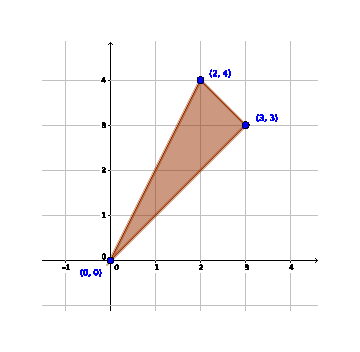
\includegraphics[width=0.45\textwidth]{ex4.pdf}
		}
		\quad
		\subcaptionbox{Exerc\'{\i}cio 5\label{fig:5}}[0.45\textwidth]{%
			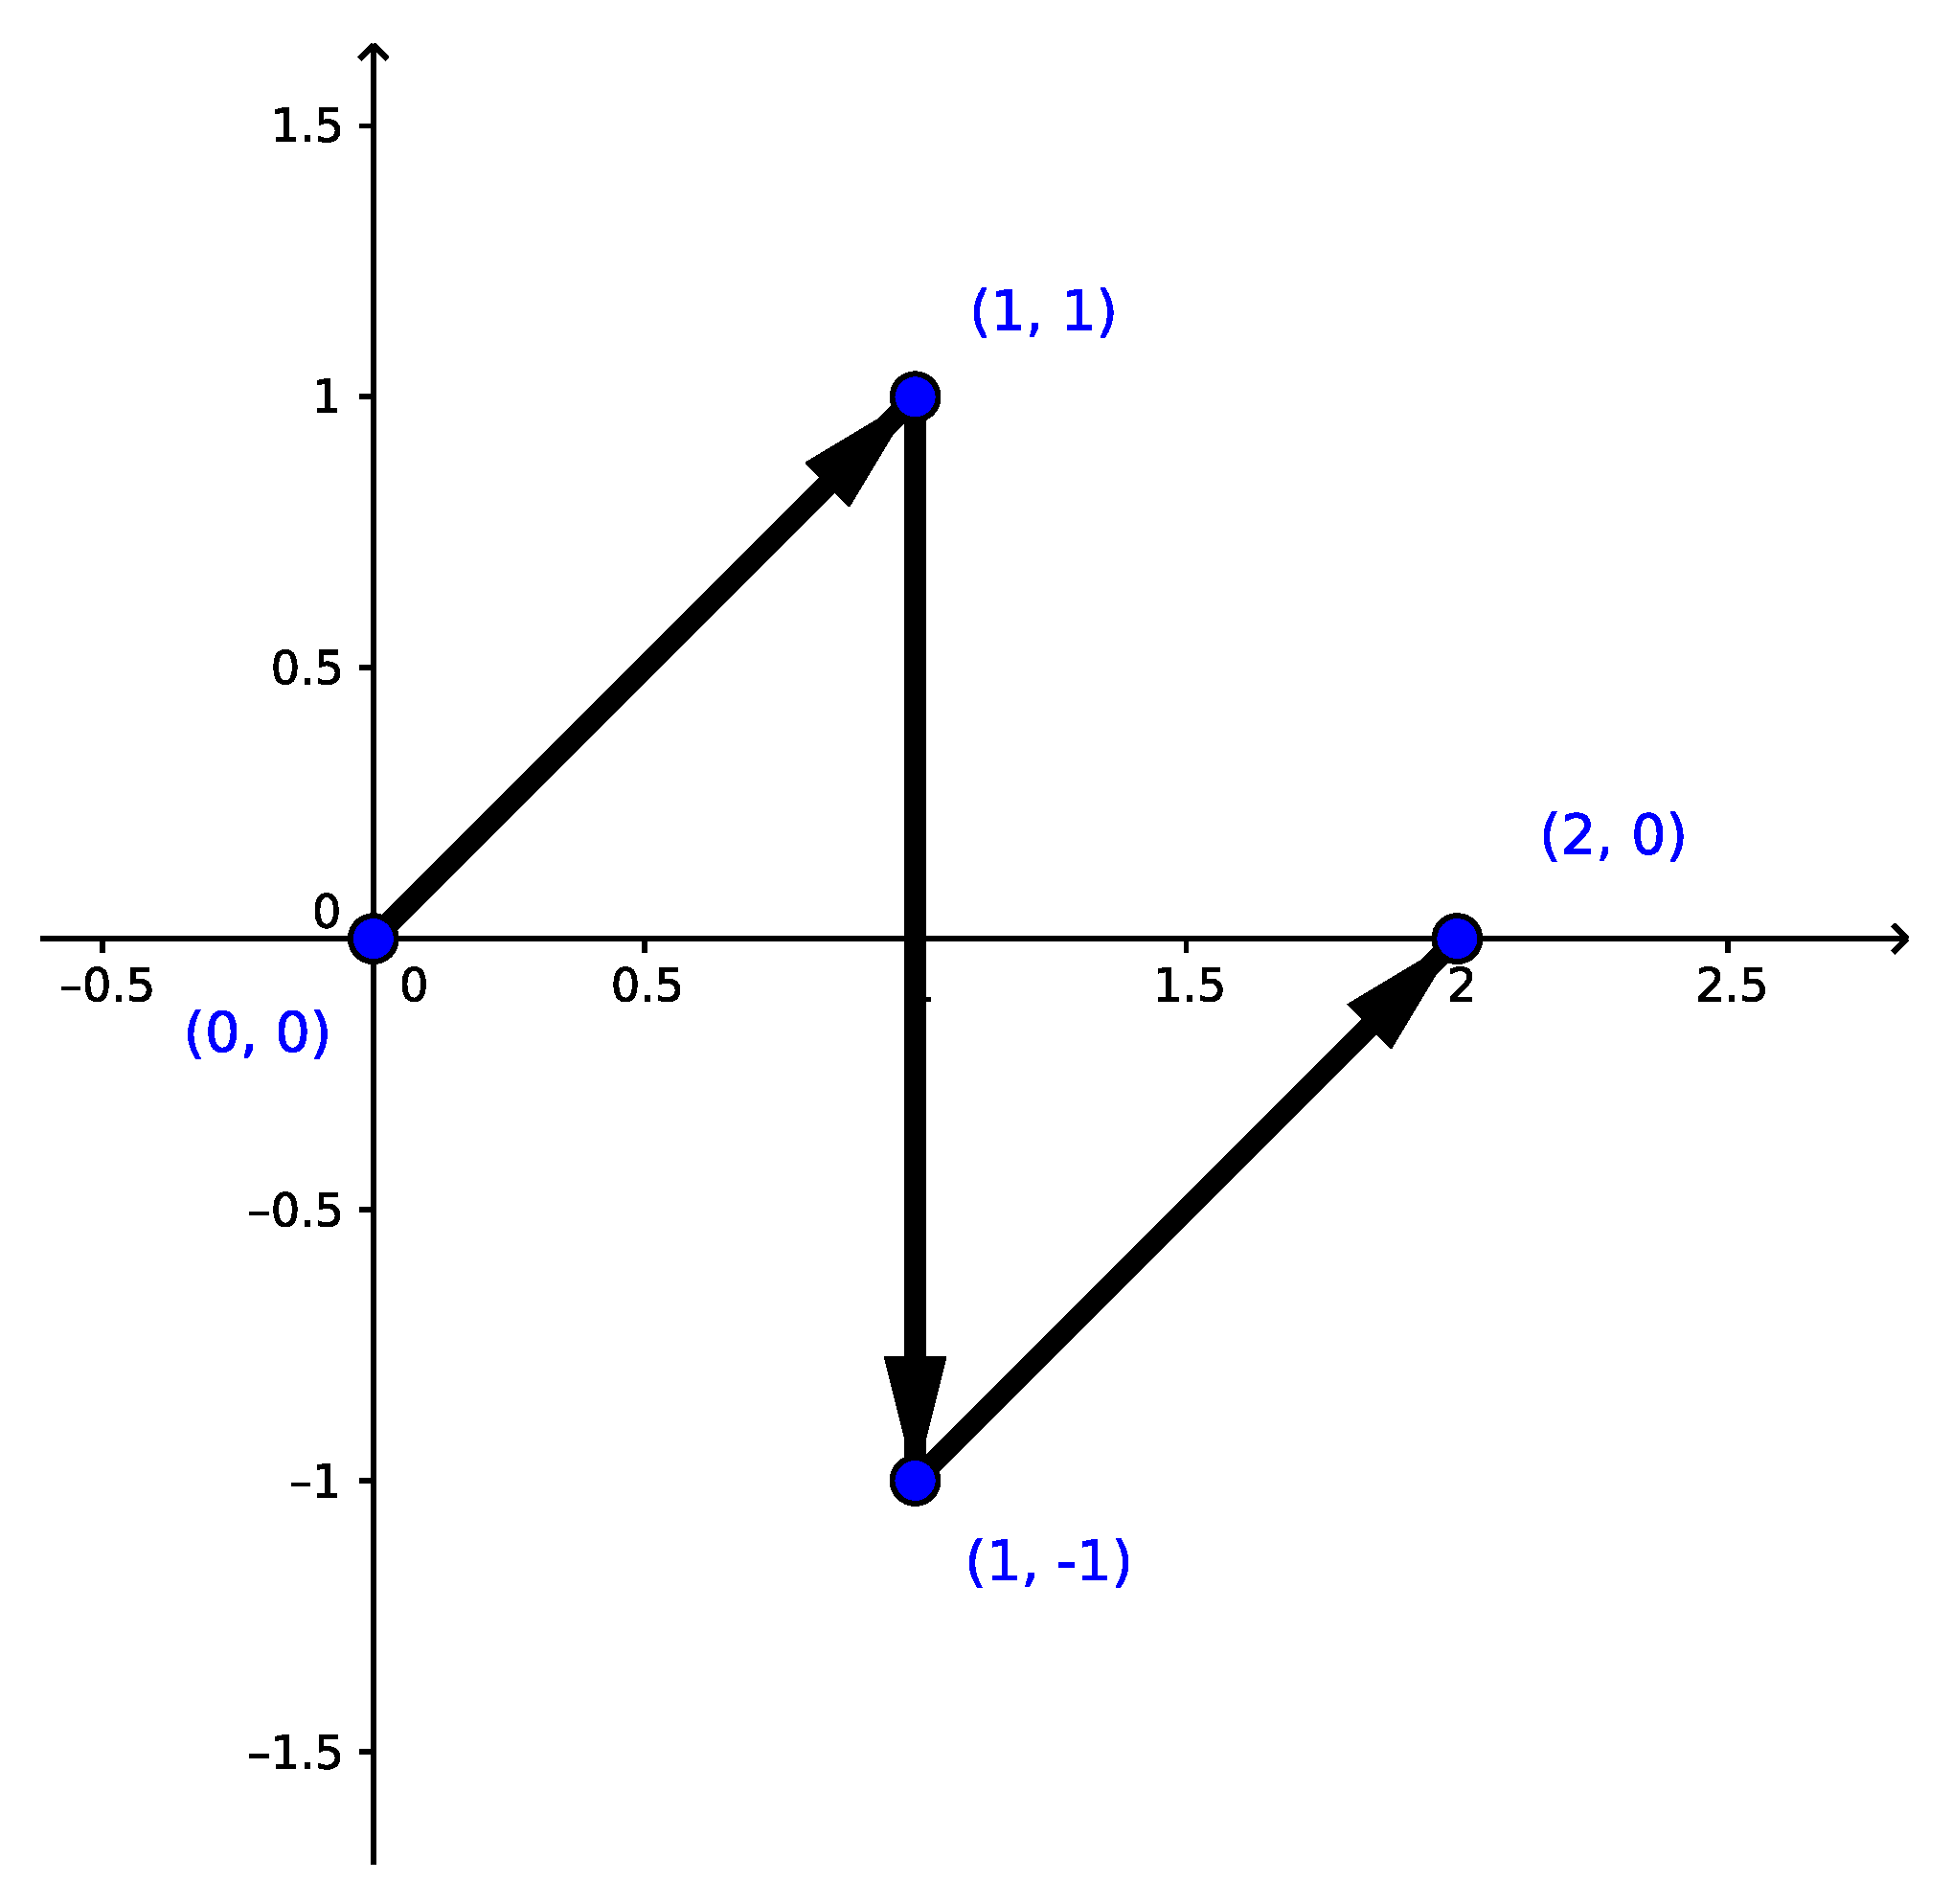
\includegraphics[width=0.45\textwidth]{ex5.pdf}
		}
	\end{figure}
\end{enumerate}

\begin{flushright}
	\textit{Boa Prova!}
\end{flushright}

\end{document}
